%This file contains the LaTeX code of my laboratory report for my Database course.
%Author: 周芯怡/Xinyi Zhou <17307130354@fudan.edu.cn>
%Author: 张作柏/Zuobai Zhang <17300240035@fudan.edu.cn>

\section{ER图与关系模式设计}

\subsection{ER图}

本项目设计的ER图如下:

\begin{figure}[h]
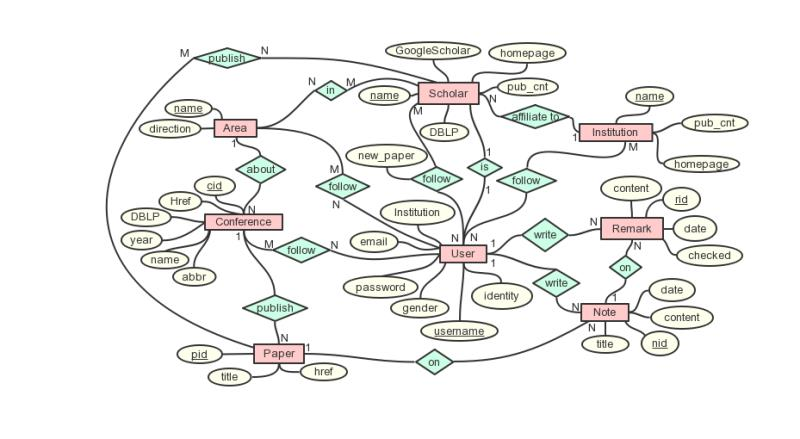
\includegraphics[width=\linewidth]{asset/ER.jpg}
\end{figure}

\subsection{关系模式与建表语句}
根据以上ER图,我们建立以下关系模式:
\begin{itemize}
\item {\myfont Institution(\uline{name}, homepage, pub\_cnt)}
\begin{lstlisting}[language=SQL]  
create table Institution(
	name char(30),
	homepage char(200),
	pub_cnt integer default 0,
	primary key(name)
	)
\end{lstlisting}
\item {\myfont Scholar(\uline{name}, homepage, DBLP, GoogleScholar, \uwave{affliliation}, pub\_cnt)}
\begin{lstlisting}[language=SQL]  
create table Scholar(
	name char(30),
	homepage  char(200),
	DBLP char(200),
	GoogleScholar char(200),
	affiliation char(30)
	pub_cnt integer default 0,
	primary key(name),
	foreign key(affiliation) references Institution(name)
	)
\end{lstlisting}
\item {\myfont Profile(\uline{username}, \uwave{scholar}, gender, identity, institution, password, email)}
\begin{lstlisting}[language=SQL]  
create table Profile(
	username char(200),
	email char(200),
	password char(200),
	scholar char(30),
	gender char(10),
	identity char(10),
	institution char(30),
	primary key(username),
	foreign key(scholar) references Scholar(name)
	)
\end{lstlisting}
\item {\myfont Conference(\uline{cid}, name, abbr, year, DBLP, Href)}
\begin{lstlisting}[language=SQL]  
create table Conference(
	cid integer,
	name char(50),
	abbr char(10),
	year integer,
	DBLP char(200),
	Href char(200),
	primary key(cid)
	)
\end{lstlisting}
\item {\myfont Paper(\uline{pid}, title, href, \uwave{conf\_id})}
\begin{lstlisting}[language=SQL]  
create table Paper(
	pid integer,
	title char(100),
	href char(500),
	conf_id integer,
	primary key(pid),
	foreign key(conf_id) references Conference(cid)
	)
\end{lstlisting}
\item {\myfont Area(\uline{name}, direction)}
\begin{lstlisting}[language=SQL] 
create table Area(
	name char(50),
	direction char(50),
	primary key(name)
	)
\end{lstlisting}
\item {\myfont Scholar\_Paper(\buline{\tuwave{scholar\_name}, \tuwave{paper\_title}})}
\begin{lstlisting}[language=SQL]  
create table Scholar_Paper(
	scholar_name char(30),
	paper_title integer,
	primary key(scholar_name, paper_title),
	foreign key(scholar_name) references Scholar(name),
	foreign key(paper_title) references Paper(pid)
	)
\end{lstlisting}
\item {\myfont Scholar\_Area(\buline{\tuwave{scholar\_name}, \tuwave{area}})}
\begin{lstlisting}[language=SQL]  
create table Scholar_Area(
	scholar_name char(30),
	area char(50),
	primary key(scholar_name, area),
	foreign key(scholar_name) references Scholar(name),
	foreign key(area) references Area(name)
	)
\end{lstlisting}
\item {\myfont Conference\_Area(\buline{\tuwave{conf\_id}, \tuwave{area}})}
\begin{lstlisting}[language=SQL]  
create table Conference_Area(
	conf_id integer,
	area char(50),
	primary key(conf_id),
	foreign key(conf_id) references Conference(cid),
	foreign key(area) references Area(name)
	)
\end{lstlisting}
\item {\myfont User\_Institution(\buline{\tuwave{user}, \tuwave{ins}})}
\begin{lstlisting}[language=SQL] 
create table User_Institution(
	user char(200),
	ins char(30),
	primary key(user, ins)
	foreign key(user) references Profile(username),
	foreign key(ins) references Institution(name)
	)
\end{lstlisting}
\item {\myfont User\_Conference(\buline{\tuwave{user}, \tuwave{conf}})}
\begin{lstlisting}[language=SQL]  
create table User_Conference(
	user char(200),
	conf integer,
	primary key(user, conf),
	foreign key(user) references Profile(username),
	foreign key(conf) references Conference(cid)
	)
\end{lstlisting}
\item {\myfont User\_Area(\buline{\tuwave{user}, \tuwave{area}})}
\begin{lstlisting}[language=SQL]  
create table User_Area(
	user char(200),
	area char(50),
	primary key(user, area),
	foreign key(user) references Profile(username),
	foreign key(area) references Area(name)
	)
\end{lstlisting}
\item {\myfont User\_Scholar(\buline{\tuwave{user}, \tuwave{sch}}, new\_paper)}
\begin{lstlisting}[language=SQL]  
create table User_Scholar(
	user char(200),
	sch char(30),
	new_paper boolean default False,
	primary key(user, sch),
	foreign key(user) references Profile(username),
	foreign key(sch) references Scholar(name)
	)
\end{lstlisting}
\item {\myfont Note(\uline{nid}, title, content, date, \uwave{author}, \uwave{paper})}
\begin{lstlisting}[language=SQL]  
create table Note(
	nid integer,
	title char(100),
	content text,
	date date,
	author char(200),
	paper integer,
	primary key(nid),
	foreign key(author) references Profile(username),
	foreign key(paper) references Paper(pid)
	)
\end{lstlisting}
\item {\myfont Remark(\uline{rid}, content, date, \uwave{author}, \uwave{note}, checked)}
\begin{lstlisting}[language=SQL]  
create table Remark(
	rid integer,
	content text,
	date date,
	author char(200),
	note integer,
	checked boolean default FALSE,
	primary key(rid),
	foreign key(author) references Profile(username),
	foreign key(note) references Note(nid)
	)
\end{lstlisting}
\end{itemize}

\subsection{函数依赖与范式分析}

{\bf 关系模式Conference}中除了非主属性对主键cid的函数依赖,还有:name→abbr,abbr→name。
形成abbr和name的传递依赖,所以只是第二范式。为了提升查询效率,我们保留了此处冗余。如果按照以下方式分解,则可以达到第三范式:\\
{\myfont Conference(name, year, DBLP, Href) \\
name\_abbr(name, abbr)}

{\bf 其余关系模式}中均只存在非主属性对主键的函数依赖,因此都是第三范式。